\chapter{Algorithms}

To further investigate the relationship between audio features, region, and song popularity, several machine learning algorithms were applied to the dataset. The goal was to build a model that could predict whether a song would be popular or not based on its audio features and release region. The following algorithms were used in this project:

\begin{itemize}
    \item Logistic Regression
    \item Decision Tree
    \item Random Forest
    \item Naive Bayes
    \item K-Nearest Neighbors
\end{itemize}

The initial steps were the same for all algorithms.

\subsection{Implementation Steps}
\begin{itemize}
    \item \textbf{Data Preparation: } The dataset is split into X and Y: X containing the audio features and region, and Y containing the popularity column.
    The popularity column is used as the target variable. Then the dataset is split into training and testing sets using an 80/20 partition.
    \item \textbf{Feature Scaling: } The features are scaled using the \textit{StandardScaler} from the \textit{sklearn.preprocessing} library. The data is normalized to ensure that all feautres contribute equally to the distance calculation involved in the model, which helps improve the convergence of the algorithm.
    \item \textbf{Handling Class Imbalancae: } To address potential class imbalance in the dataset, the \textit{Synthetic Minority Over-sampling Technique (SMOTE)} was applied, which
    created synthetic samples of the minorty class (popular songs). 
    %was this used for all models?
    \item \textbf{Model Training: } The algorithm models were trained using the scaled training set. The model was
    configured with a maximum iteration limit of 2000 and class weight balanced to give equal importance to both classes during the training.
    \item \textbf{Cross-Validation: } To evaluate the model's performance more robustly, 5-fold cross-validation was performed.
    This technique involves splitting the data into five subsets (folds) and training the model on four folds while validating it on the remaining
    fold. This process is repeated five times, each time using a different fold for validation.
    \item \textbf{Predictions: } Predictions were made on the scaled test set, and probabilities were calculated for class membership. A threshold of 0.3 was used to adjust the predicted probabilities to determine class labels.
    \item \textbf{Model Evaluation: } The model was evaluated using the confusion matrix, classification report, which included metrics such as precicion, recall, and F1-score.
    \item \textbf{Feature Importance: } The feature importance of the model was determined by examining the coefficients of the models. Both feature importance for the whole dataset and feature importance for each specific region has been applied. As a result, dominant features to determine the populartiy of the songs were found.
    \item \textbf{Regional Analysis: } Regional analysis was performed to better understand how different audio features contribute to make a song popular across various regions.
\end{itemize} 


\newpage


\section{Logistic Regression}
Logistic regression a supervised machine learning algorithm that is used to
compute classification problems with a binary output.
It is based on the idea of modeling the probability of a certain class or event.
Unlike linear regression, which predicts continuous values, logistic regression predicts categorical outcomes by applying a logistic function to the input data.
In this case, it's used to predict
whether a song will be popular or not, depending on the region and the 
audio features of the song. The output is
either 0 or 1, whith 0 representing the song most probably will not be popular and 
1 representing the song most probably will be popular. \\



Accuracy: \textbf{85.42\%}

% Confusion Matrix
% \begin{table}[h]
%     \centering
%     \begin{tabular}{cc|c|c|}
%         \toprule
%         & & \multicolumn{2}{c}{Predicted} \\
%         \cline{3-4}
%         & & 0 & 1 \\
%         \hline
%         \multirow{2}{*}{\textbf{Actual}} & 0 & 55340 & 0 \\
%         & 1 & 9613 & 0 \\
%         \bottomrule
%     \end{tabular}
%     \caption{Confusion Matrix}
%     \label{tab:confusion_matrix}
% \end{table}

Classification Report
\begin{table}[h]
    \centering
    \begin{tabular}{lcccc}
        \toprule
        & \textbf{Precision} & \textbf{Recall} & \textbf{F1-score} & \textbf{Support} \\
        \midrule
        0 & 0.85 & 1.00 & 0.92 & 55340 \\
        1 & 0.00 & 0.00 & 0.00 & 9613 \\
        \midrule
        \textbf{Accuracy} & \multicolumn{4}{c}{0.85} \\
        \textbf{Macro avg} & 0.43 & 0.50 & 0.46 & 64953 \\
        \textbf{Weighted avg} & 0.73 & 0.85 & 0.78 & 64953 \\
        \bottomrule
    \end{tabular}
    \caption{Classification Report}
    \label{tab:classification_report}
\end{table}

\begin{figure}[h] 
    \centering 
    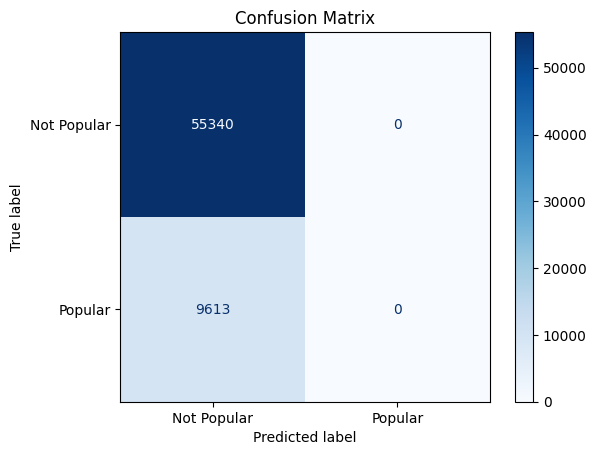
\includegraphics[width=0.6\textwidth]{media/log_reg_confusionmatrix.png}
    \caption{Confusion Matrix of Logistic Regression Model}

\end{figure}

Despite having a strong accuracy, the confusion matrix shows that the model is not able to predict correctly when a song will be popular. This is due to the class imbalance in the dataset, where the number of non-popular songs is significantly higher than the number of popular songs. As a result, the model tends to predict non-popular songs more frequently, leading to a high number of false negatives. 
%This issue can be addressed by using techniques such as oversampling or undersampling to balance the classes in the dataset.


\newpage

\section{Decision Tree}

Decision Tree is a supervised machine learning algorithm that is used for both classification and regression tasks. It works by recursively partitioning the data into subsets based on the values of the input features. The goal is to create a model that predicts the value of the target variable by learning simple decision rules inferred from the data features. Decision trees are easy to interpret and visualize, making them popular for exploratory data analysis and decision-making tasks. In this project, Decision Tree was used to predict whether a song will be popular or not based on their audio features and region affiliation. \\

After splitting the dataset into test and train sets and fitting the model, the Decision Tree model was evaluated using the following metrics: accuracy, confusion matrix and classification report.


Accuracy: \textbf{75.97\%}

Classification Report
\begin{table}[h]
    \centering
    \begin{tabular}{lcccc}
        \toprule
        & \textbf{Precision} & \textbf{Recall} & \textbf{F1-score} & \textbf{Support} \\
        \midrule
        0 & 0.87 & 0.85 & 0.86 & 55340 \\
        1 & 0.22 & 0.25 & 0.23 & 9613 \\
        \midrule
        \textbf{Accuracy} & \multicolumn{4}{c}{0.76} \\
        \textbf{Macro avg} & 0.54 & 0.55 & 0.55 & 64953 \\
        \textbf{Weighted avg} & 0.77 & 0.76 & 0.77 & 64953 \\
        \bottomrule
    \end{tabular}
    \caption{Classification Report}
    \label{tab:classification_report}
\end{table}
 
\begin{figure}[h] 
    \centering 
    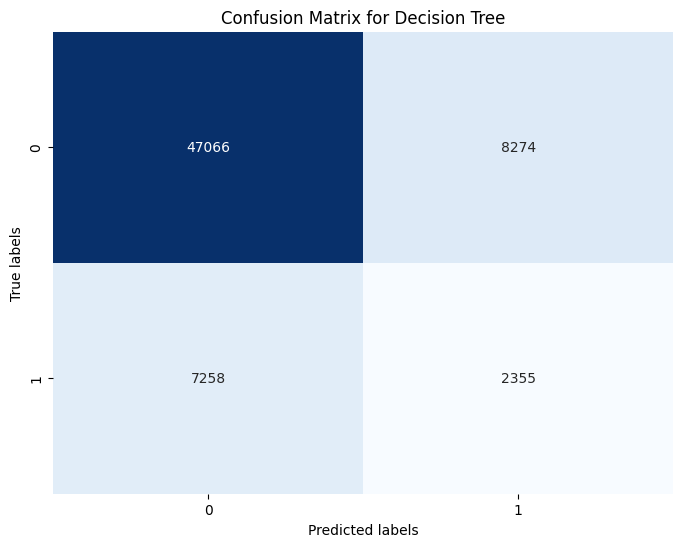
\includegraphics[width=0.6\textwidth]{media/decision_tree_conf_matr.png}
    \caption{Confusion Matrix of Decision Tree Model}

\end{figure}

The Decision Tree model has a lower accuracy compared to the Logistic Regression model, but the confusion matrix shows a better balance between the number of true positives and true negatives. This indicates that the Decision Tree model is better at predicting both popular and non-popular songs. However, the model still struggles with class imbalance, as evidenced by the low recall and precision values for the positive class. %This issue can be addressed by using techniques such as oversampling or undersampling to balance the classes in the dataset.

\newpage
The Decision Tree Classifier can be shown:

\begin{figure}[H] 
    \centering 
    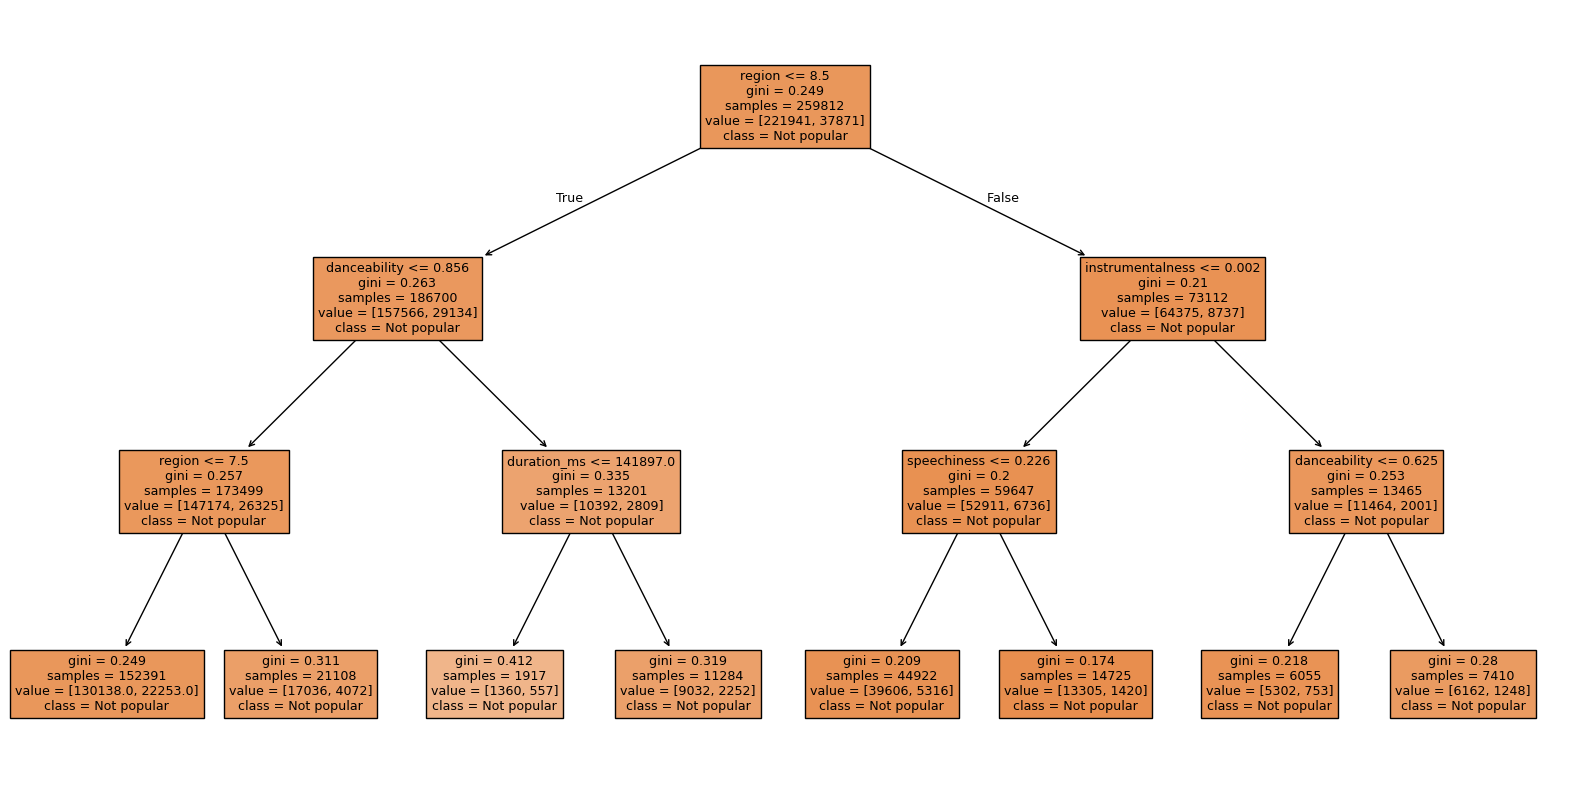
\includegraphics[width=0.9\textwidth]{media/decision_tree.png}
    \caption{Decision Tree Classifier}
    \label{fig:decision_tree}
\end{figure}



\section{Random Forest}
Random Forest is an ensemble learning method that constructs a multitude of decision trees during
training and outputs the mode of the classes as the prediction of the individual trees. It can be used for both classification and regression
tasks. Random Forest
is known for its robustness, scalability, and ability to handle high-dimensional data with ease.
In this project, Random Forest was used to predict whether the song will be popular or not based on their audio
features and region affiliation. \\
The concept of Random Forest is based on Bagging (Bootsrap Aggregating) which is a technique used to reduce the variance of the model
by averaging the predictions of multiple models. Random Forest builds multiple decision trees and merges them together to get a more
accurate and stable prediction.
\\
\\
Mathematically, if \( T_1, T_2, \dots, T_B \) are the \( B \) decision trees in the forest, and \( h(x) \) is the output prediction of a single tree for input \( x \), the Random Forest prediction for classification is:

\[
\hat{y} = \text{mode} \left( T_1(x), T_2(x), \dots, T_B(x) \right)
\]

For the regression, the final prediction is the average:

\[
\hat{y} = \frac{1}{B} \sum_{i=1}^{B} T_i(x)
\]
\\
\\
\\
Accuracy: \textbf{85.67\%}

\newpage
Classification Report
\begin{table}[h]
    \centering
    \begin{tabular}{lcccc}
        \toprule
        & \textbf{Precision} & \textbf{Recall} & \textbf{F1-score} & \textbf{Support} \\
        \midrule
        0 & 0.88 & 0.96 & 0.92 & 55340 \\
        1 & 0.53 & 0.26 & 0.35 & 9613 \\
        \midrule
        \textbf{Accuracy} & \multicolumn{4}{c}{0.86} \\
        \textbf{Macro avg} & 0.71 & 0.61 & 0.64 & 64953 \\
        \textbf{Weighted avg} & 0.83 & 0.86 & 0.84 & 64953 \\
        \bottomrule
    \end{tabular}
    \caption{Classification Report}
    \label{tab:classification_report}
\end{table}

\begin{figure}[h] 
    \centering 
    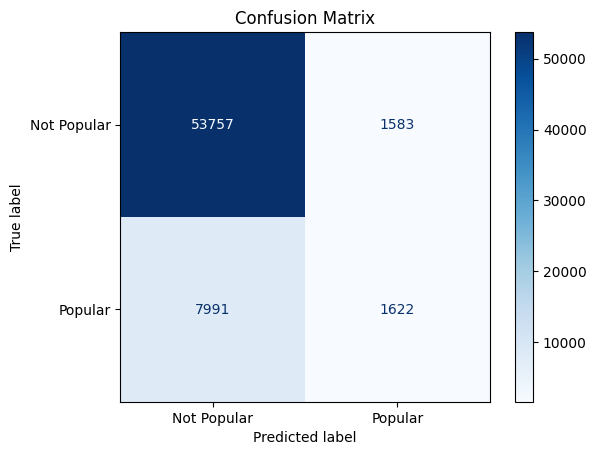
\includegraphics[width=0.6\textwidth]{media/random_forest_conf_matrix.png}
    \caption{Confusion Matrix of Random Forest Model}

\end{figure}

In this case there's both a good accuracy of the model and a good result of the confusion matrix, which shows a better balance between the number of true positives and true negatives. This is why the Random Forest model is the one taken into account for the final results.

\section{Naïve Bayes}
Naïve Bayes is a family of probabilistic algorithms based on Bayes' Theorem, which is used for classification tasks.
The algorithm is particularly popular for its simplicity, efficiency, and effectiveness in dealing with large datasets.
It is called "naïve" because it makes the assumption that the features are independent from each other given the class label.
In this project Gaussian Naive Bayes is used to predict whether a song will be popular or not based on its audio features and release region by assuming that
the features follow a normal distribution. 

The Bayes' Theorem is expressed as:

\[
P(C | X) = \frac{P(X | C) \cdot P(C)}{P(X)}
\]

Where:
\begin{itemize}
    \item \( P(C | X) \) is the posterior probability of class \( C \) given the features \( X \).
    \item \( P(X | C) \) is the likelihood of observing the features \( X \) given class \( C \).
    \item \( P(C) \) is the prior probability of class \( C \).
    \item \( P(X) \) is the prior probability of observing the features \( X \).
\end{itemize}

To make predictions, Naïve Bayes calculates the posterior probability for each class and selects the class with the highest probability. The independence assumption simplifies the calculation of the likelihood:

\[
P(X | C) = P(X_1 | C) \cdot P(X_2 | C) \cdots P(X_n | C)
\]

Where \( X_1, X_2, \ldots, X_n \) are the features.

Accuracy: \textbf{85.04\%}


Classification Report
\begin{table}[h]
    \centering
    \begin{tabular}{lcccc}
        \toprule
        & \textbf{Precision} & \textbf{Recall} & \textbf{F1-score} & \textbf{Support} \\
        \midrule
        0 & 0.85 & 1.00 & 0.92 & 55340 \\
        1 & 0.17 & 0.00 & 0.01 & 9613 \\
        \midrule
        \textbf{Accuracy} & \multicolumn{4}{c}{0.85} \\
        \textbf{Macro avg} & 0.51 & 0.50 & 0.46 & 64953 \\
        \textbf{Weighted avg} & 0.75 & 0.85 & 0.78 & 64953 \\
        \bottomrule
    \end{tabular}
    \caption{Classification Report}
    \label{tab:classification_report}
\end{table}

\begin{figure}[h] 
    \centering 
    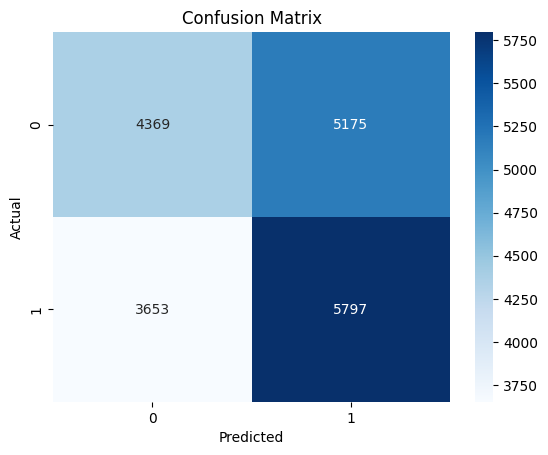
\includegraphics[width=0.6\textwidth]{media/naive_bayes_confusion_matrix.png}
    \caption{Confusion Matrix of Naive Bayes Model}

\end{figure}

Also in this case the accuracy is good, but the confusion matrix shows that the model is not able to predict correctly when a song will be popular. As a result, the model tends to predict non-popular songs more frequently, leading to a high number of false negatives.

\newpage


\section{K-Nearest Neighbors}

K-Nearest Neighbors (KNN) is a simple, instance-based learning algorithm that is used for classification and regression tasks. It is a non-parametric method that makes predictions based on the similarity of the input data to the training data. KNN is a lazy learning algorithm, meaning that it does not learn a model during training but instead stores the training data and makes predictions at runtime. The algorithm works by calculating the distance between the input data and the training data and selecting the K-nearest neighbors to make a prediction. The class label of the majority of the neighbors is assigned to the input data as the predicted class. In this project, KNN was used to predict whether a song will be popular or not based on its audio features and region affiliation. \\

Accuracy: \textbf{83.92\%}


Classification Report
\begin{table}[h]
    \centering
    \begin{tabular}{lcccc}
        \toprule
        & \textbf{Precision} & \textbf{Recall} & \textbf{F1-score} & \textbf{Support} \\
        \midrule
        0 & 0.87 & 0.96 & 0.91 & 55340 \\
        1 & 0.39 & 0.16 & 0.22 & 9613 \\
        \midrule
        \textbf{Accuracy} & \multicolumn{4}{c}{0.85} \\
        \textbf{Macro avg} & 0.63 & 0.56 & 0.57 & 64953 \\
        \textbf{Weighted avg} & 0.80 & 0.84 & 0.81 & 64953 \\
        \bottomrule
    \end{tabular}
    \caption{Classification Report}
    \label{tab:classification_report}
\end{table}

\begin{figure}[h] 
    \centering 
    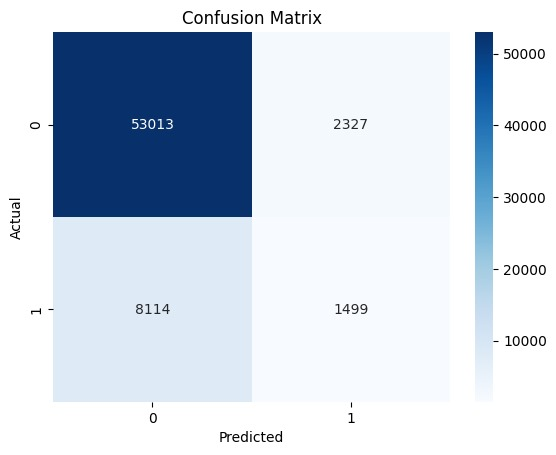
\includegraphics[width=0.6\textwidth]{media/knn-confusion_matrix.jpg}
    \caption{Confusion Matrix of KNN Model}

\end{figure}

\newpage

The KNN algorithm allows us to calculate and plot the ROC curve, which is a graphical representation of the true positive rate against the false positive rate. This is useful for evaluating the performance of a classification model and comparing different models. The area under the ROC curve (AUC) is a measure of the model's ability to distinguish between the classes. A higher AUC value indicates a better-performing model.\\
The True Positive Rate (Sensitivity/Recall) on the y-axis shows how often the model correctly identifies a popular song (i.e., correctly predicts a "positive" class).\\
The False Positive Rate on the x-axis shows how often the model incorrectly predicts a song as popular when it's not (i.e., incorrectly predicts a "positive" class when it should have been negative).\\
The red dashed line represents a random classifier, meaning if the model was making random predictions, the ROC curve would follow this line (AUC = 0.5).\\
The ROC curve for the KNN model is shown below:

\begin{figure} [H]
    \centering
    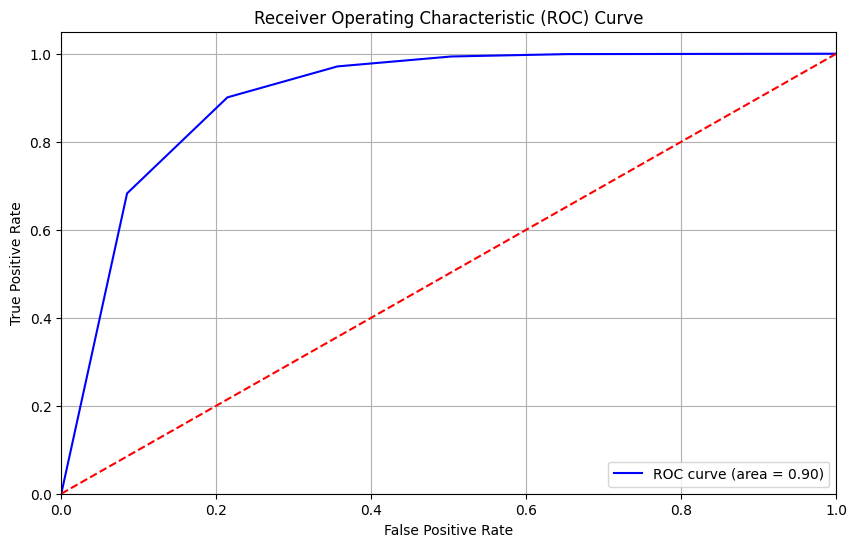
\includegraphics[width=0.6\textwidth]{media/roc_curve.png}
    \caption{ROC Curve of KNN Model}
    \label{fig:knn_roc_curve}
\end{figure}

An AUC of 0.63 suggests that the KNN model is performing better than random, but it is still relatively weak.
A perfect model would have an AUC of 1.0, where it correctly distinguishes between popular and non-popular songs without error.

This means that it is able to capture some patterns in the data, but the performance is not particularly strong. 